\documentclass[11pt]{article}

\usepackage[hidelinks]{hyperref}

\usepackage[scaled]{helvet}
\usepackage[T1]{fontenc}
\renewcommand\familydefault{\sfdefault}

\usepackage[margin=1in]{geometry}

\usepackage[utf8]{inputenc}

\usepackage{amsmath}
\usepackage{algorithm}
\usepackage[noend]{algpseudocode}
\algnewcommand\algorithmicforeach{\textbf{parallel for each}}
\algdef{S}[FOR]{ForEach}[1]{\algorithmicforeach\ #1\ \algorithmicdo}

\algnewcommand\algorithmicinput{\textbf{Input:}}
\algnewcommand\algorithmicoutput{\textbf{Output:}}
\algnewcommand\Input{\item[\algorithmicinput]}%
\algnewcommand\Output{\item[\algorithmicoutput]}%
\algnewcommand{\lIf}[2]{% \IfThen{<if>}{<then>}
  \State \algorithmicif\ #1\ \algorithmicthen\ #2}

\usepackage{graphicx}
\usepackage{subcaption}
\usepackage[justification=centering]{caption}

\usepackage{cite}

\usepackage{amsthm}

\usepackage{xcolor}

\newcommand{\blue}[1]{\textcolor{blue}{#1}}

\newcommand{\red}[1]{\textcolor{red}{#1}}

\title{Induced 6-Cycle Counting in Bipartite Graphs}

\begin{document}
 
\author{
Jason Niu \\
jasonniu@buffalo.edu
}
\date{}

\maketitle

\begin{abstract}
Finding subgraphs in a bipartite graph is crucial to understanding its underlying structure.
The smallest non-trivial subgraph in a bipartite graph is a 4-cycle, which is also known as a butterfly.
Shi and Shun recently used the affordances of parallelization to develop efficient butterfly counting algorithms.
However, parallel approaches to counting larger cycles is a relatively unexplored area.
In this paper, we propose a parallel algorithm for efficiently counting induced 6-cycles.
\end{abstract}

\section{Introduction}
Many real-world networks are represented by a bipartite graph.
For example, recommendation networks often are represented as a bipartite graph with users on one partition and items on the other \cite{li2013recommendation}.
Finding graph motifs that form the building blocks of these networks can reveal the underlying structure within bipartite graphs.

In unipartite graphs, the smallest cycle is a 3-cycle, which is also known as a triangle.
However, since bipartite graphs contain no odd cycles, triangles do not exist in bipartite graphs.
The smallest cycle in a bipartite graph is a 4-cycle, which is also known as a butterfly.
Butterflies are the smallest building blocks for community structures in bipartite graphs.

\begin{figure}[h]
    \centering
    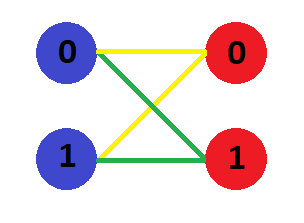
\includegraphics[width=0.25\textwidth]{figures/Butterfly.png}
    \caption{\small This graph depicts a butterfly. Nodes in u are in blue while nodes in v are in red. The butterfly is made of two wedges, which are highlighted in yellow and green.}
    \label{fig:butterfly}
\end{figure}

Counting cycles in bipartite graphs is NP-hard \cite{flum2004parameterized}.
Sequential algorithms for butterfly counting use the concept of combining wedges (2-paths) to count butterflies (see Figure \ref{fig:butterfly}) ~\cite{wang2014rectangle, sanei2018butterfly, chiba1985arboricity}.
When dealing with larger graphs, however, the runtime of sequential algorithms may be problematic.
Adapting sequential algorithms for parallelization can significantly reduce the runtime of these algorithms.
Shi and Shun \cite{shi2019parallel} recently designed a parallel butterfly counting algorithm which modified Chiba and Nishizeki's wedge retrieval process \cite{chiba1985arboricity} to enable parallelization.

\begin{figure}[h]
    \centering
    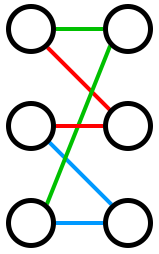
\includegraphics[width=0.1\textwidth]{figures/Triangle.png}
    \caption{\small In this figure, a triangle of wedges (colored as red, blue, and green) forms a 6-cycle.}
    \label{fig:triangle}
\end{figure}

Given the relevance of bipartite graphs in real-world relationships, it is desirable to find larger cycles within these graphs.
Karimi and Banihashemi \cite{karimi2012message} designed a message-passing algorithm for counting cycles of length \textit{g} to \textit{2g-2} in bipartite graphs, where \textit{g} is the girth of the graph.
Dehghan and Banihashemi \cite{dehghan2019counting} proposed an algorithm that uses breadth-first search to count cycles of length \textit{g}  to \textit{g+4} in bipartite graphs.
However, these sequential algorithms have only been tested on small bipartite graphs.

\begin{figure}[h]
    \centering
    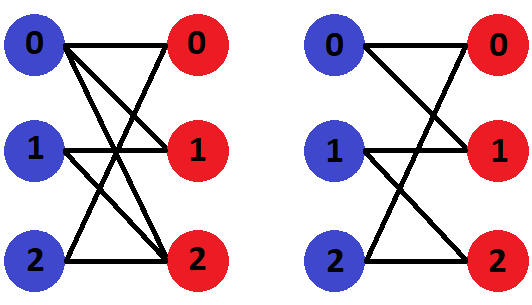
\includegraphics[width=0.25\textwidth]{figures/Induced vs Noninduced.png}
    \caption{\small The graph on the left depicts a non-induced 6-cycle. The graph on the right depicts an induced 6-cycle. In the non-induced graph, the removal of the edge from \blue{0} to \red{2} won't affect the 6-cycle.}
    \label{fig:induced}
\end{figure}

Recently, Yang et al. introduced sequential algorithms for counting non-induced 6-cycles in large bipartite networks \cite{yang2020efficient}.
Their algorithms are based on the concept that a 6-cycle is a triangle of wedges (see Figure \ref{fig:triangle}) or a pair of 3-paths.
In this paper, we propose a parallel algorithm that is also based on the concept that an 6-cycle is a triangle of wedges.
Parallelizing algorithms that count larger cycles is extremely valuable due to their increased complexity.
This paper presents a framework for counting induced 6-cycles (see Figure \ref{fig:induced}) in bipartite graphs which uses the affordances of parallelization to maximize efficiency.

\section{Notation}
We work on a simple and undirected bipartite graph \textit{G = (U, V, E)} where \textit{U} is the set of nodes in the left set, \textit{V} is the set of nodes in right set, and \textit{E} is the set of edges.
The neighbors of a node \textit{v} is denoted by \textit{N(v)}.
A \textbf{wedge} is a set of three nodes \textit{u1, u2} $\in$ \textit{U} and \textit{v} $\in$ \textit{V} composed of edges \textit{(u1, v), (u2, v)} $\in$ \textit{E}. 
We call the nodes \textit{u1, u2} \textbf{endpoints} and the node \textit{v} the \textbf{center}.
An \textbf{induced 6-cycle} is a set of six nodes \textit{u1, u2, u3} $\in$ \textit{U} and \textit{v1, v2, v3} $\in$ \textit{V} such that its internal edges exactly form a cycle.

\section{Algorithm}

We introduce a parallel algorithm for counting induced 6-cycles in bipartite graphs.
Our algorithm extends the parallel wedge retrieval algorithm proposed by Shi and Shun \cite{shi2019parallel}.

\setlength{\textfloatsep}{0pt}
\begin{algorithm}[H]
\caption{\textsc{Preprocessing($G = (U, V, E)$)}}
\label{alg:Preprocessing}
\begin{algorithmic}[1]
    \Input $G$: graph
    \Output $G'$: ordered graph
        \State $w_u \gets 0$
        \ForEach {$x \in U$}
            \State $n \gets |G(x)|$
            \State $w_u \gets w_u + \frac{n * (n - 1)}{2}$
        \EndFor
        \State $w_v \gets 0$
        \ForEach {$x \in V$}
            \State $n \gets |G(x)|$
            \State $w_v \gets w_v + \frac{n * (n - 1)}{2}$
        \EndFor
        \If{$w_u < w_v$}
            \State $Swap(U, V)$ \Comment swap $U$ and $V$
        \EndIf
        \State $X \gets Sort(U)$ \Comment sort $U$ in increasing order of degree
        \State Let $x$'s rank $R(x)$ be its index in $X$
        \ForEach {$x \in U \cup V$}
            \If{$x \in U$}
                \State $G'(R(x)) \gets \{y | (x, y) \in E\}$
            \Else
                \State $G'(x) \gets Sort(\{R(y) | (x, y) \in E\})$ \Comment sort neighbors' ranks by descending order
            \EndIf
        \EndFor
        \State \textbf{return} $G'$
\end{algorithmic}
\end{algorithm}

We give a preprocessing algorithm (Algorithm \ref{alg:Preprocessing}) that takes as input a bipartite graph, swaps left and right sets depending on their wedge counts, and renames nodes in increasing order of degree.
\textit{Preprocessing} swaps $U$ and $V$ if the number of wedges whose center is $\in$ $U$ is less than the number of wedges whose center is $\in$ $V$.
This helps reduce the number of processed wedges.
\textit{Preprocessing} then orders nodes in increasing order of degree, which we found to yield efficient results.
Shi and Shun \cite{shi2019parallel} proved that using approximate degree ordering, complement degeneracy ordering, and approximate complement degeneracy ordering also gives work-efficient bounds.
By establishing an ordering of nodes, we can avoid traversing the same induced 6-cycle twice.

\begin{algorithm}[H]
\caption{GetWedges(\textit{G})}
\label{alg:GetWedges}
\hspace*{\algorithmicindent} \textbf{Input:} \textit{G}: graph \\
\hspace*{\algorithmicindent} \textbf{Output:} \textit{W}: list of wedges
\begin{algorithmic}[1]
    \ForEach {$u1 \in U$}
        \ForEach {$v \in N(u1)$}
            \ForEach {$u2 \in N(v)$}
                \If{$u2 > u1$}
                    \State $W((u1, v, u2))$ \Comment add wedge to $W$
                \Else
                    \State break
                \EndIf
            \EndFor
        \EndFor
    \EndFor
    \State \textbf{return} $W$
\end{algorithmic}
\end{algorithm}

We define a wedge retrieval algorithm, $GetWedges$ (Algorithm \ref{alg:GetWedges}), that takes as input a preprocessed graph and outputs a list of wedges.
We use \textit{W} to denote a parallel container such that \textit{W(x)} stores \textit{x} in the container.
\textit{W} should allow for fast access of wedges based on endpoints such that when accessing all wedges whose smallest endpoint is $u1$ $\in$ $U$, wedges are sorted based on the other endpoint.
$GetWedges$ is based off of Shi and Shun \cite{shi2019parallel} wedge retrieval algorithm which enables the parallel processing of wedges.
For all nodes \textit{u1} $\in$ \textit{U}, the algorithm retrieves all wedges with endpoints \textit{u1, u2} and center \textit{v} such that \textit{u2} is greater than \textit{u1}.
Note that Shi and Shun proved how once we have retrieved all wedges with endpoint \textit{u1}, there is no need to consider wedges with center \textit{u1}.
Although this point was originally applied to butterfly counting, the same logic can be applied to induced 6-cycles.

\begin{algorithm}[H]
\caption{Par6CycleCount(\textit{G}, \textit{W})}
\label{alg:Par6CycleCount}
\hspace*{\algorithmicindent} \textbf{Input:} \textit{G}: graph\\
\hspace*{\algorithmicindent} \textbf{Output:} \textit{c}: count of induced 6-cycles
\begin{algorithmic}[1]
    \State $G \gets Preprocessing(G)$
    \State $W \gets GetWedges(G)$
    \State $c \gets 0$
    \ForEach {$u1 \in U$}
        \For {\textbf{each} $w1 \in W(u1)$} \Comment $u1$ is smallest endpoint in $w1$
            \State $c' \gets 0$
            \State $x, y \gets -1$
            \State $skip \gets false$
            \State $u1, v1, u2 \gets w1$
            \For {\textbf{each} $w2 \in W(u2)$} \Comment $u2$ is smallest endpoint in $w2$
                \State $u2, v2, u3 \gets w2$
                \If{$skip \cap (x = u3)$}
                    \State continue
                \EndIf
                \State $x \gets u3$
                \State $skip \gets v1 \in N(u3)$
                \If{$!skip \cap (v2 \notin N(u1))$}
                    \If{$y \neq u3$}
                        \State $c' \gets 0$
                        \For {\textbf{each} $w3 \in W(u1, u3)$} \Comment $u1, u3$ are endpoints of $w3$
                            \State $u1, v3, u3 \gets w3$
                            \If{$v3 \notin N(u2)$}
                                \State $c' \gets c' + 1$
                            \EndIf
                        \EndFor
                        \State $y \gets u3$
                    \EndIf
                    \State $c \gets c + c'$
                \EndIf
            \EndFor
        \EndFor
    \EndFor
    \State \textbf{return} $c$
\end{algorithmic}
\end{algorithm}

We now describe the induced 6-cycle counting algorithm, which is given as $Par6CycleCount$ in Algorithm \ref{alg:Par6CycleCount}.
Given a bipartite graph $G$, this algorithm applies $G$ to the preprocessing and wedge retrieval algorithms described in Algorithms \ref{alg:Preprocessing} and \ref{alg:GetWedges}, respectively.
We use $W(x)$ to denote the set of wedges where $x$ is the smallest of the two endpoints and $W(x, y)$ to denote the set of wedges whose endpoints are $x$ and $y$.
$Par6CycleCount$ finds triangles of wedges $\{u1, v1, u2\}$, $\{u2, v2, u3\}$, and $\{u1, v3, u3\}$ such that $u1 < u2 < u3$.
For every triangle of wedges, there are a maximum of three checks for inducedness (see Figure \ref{fig:inducedness}).
Inducedness checks are skipped if a similar set of wedges was processed previously (see Figure \ref{fig:speedups}).

\begin{figure}[h]
    \centering
    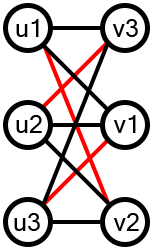
\includegraphics[width=0.1\textwidth]{figures/Inducedness.png}
    \caption{\small In this figure, the red edges prevent inducedness for the 6-cycle colored in black. Each inducedness check (lines 15, 16, and 21) in Algorithm \ref{alg:Par6CycleCount}, $Par6CycleCount$, corresponds to a red edge.}
    \label{fig:inducedness}
\end{figure}

\begin{figure}[h]
    \centering
    \begin{subfigure}{.1\textwidth}
        \centering
        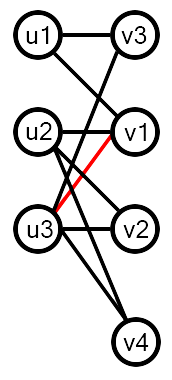
\includegraphics[height=3cm]{figures/speedup1.png}
    \end{subfigure}
    \begin{subfigure}{.1\textwidth}
        \centering
        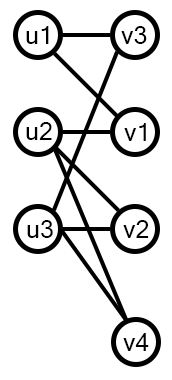
\includegraphics[height=3cm]{figures/speedup2.png}
    \end{subfigure}
    \caption{\small The speedups implemented in lines 12 (left) and 17 (right) of $Par6CycleCount$. The figure on the left shows only one inducedness check (the red edge) is needed for wedges $\{u2, v2, u3\}$ and $\{u2, v4, u3\}$. The figure on the right shows that the count of 6-cycles for wedge $\{u2, v2, u3\}$ is the same as wedge $\{u2, v4, u3\}$. Therefore, we only need to do calculations for one wedge.}
    \label{fig:speedups}
\end{figure}

\begin{proof}[Proof of correctness]
We will prove Algorithm \ref{alg:Par6CycleCount}, $Par6CycleCount$, is correct by contradiction.

Suppose there exists a set of nodes that is inaccurately counted as an induced 6-cycle.
Since lines 15, 16, and 21 check for inducedness given a set of 6 nodes, every node set counted must be an induced 6-cycle, contradicting our claim.

Suppose there exists an induced 6-cycle that is counted twice.
In Algorithm \ref{alg:GetWedges}, $GetWedges$, the ordering of node traversal in line 4 prevents a wedge from being traversed multiple times, causing each wedge to be stored only once in line 5.
There also exists a specific ordering of wedge traversal for $Par6CycleCount$ in lines 5, 10, and 19.
For every induced 6-cycle, the wedge which contains the smallest two endpoints is traversed first (line 5).
Then, the wedge containing the largest two endpoints is traversed second (line 10).
Finally, the wedge which contains the smallest and the largest endpoint is traversed last (line 19).
This prevents an induced 6-cycle from being traversed multiple times, contradicting our claim of duplicity in induced 6-cycle counting.

Suppose there exists an induced 6-cycle $x = \{u1, u2, u3, v1, v2, v3\}$ that isn't counted.
Then x contains three wedges $a = \{u1, v1, u2\}$, $b = \{u2, v2, u3\}$, and $c = \{u1, v3, u3\}$, which the algorithm processes in that order (lines 5, 10, and 19).
Therefore, the algorithm counts the triangle of wedges $a$, $b$, and $c$ as an induced 6-cycle, contradicting our claim.

Since all possible cases lead to contradiction, $Par6CycleCount$ returns the correct induced 6-cycle count.
\end{proof}

\section {Results}

In this section, we present the runtime of our algorithm on real-world datasets, whose main characteristics are shown in Table \ref{tab:datasets}.

\begin{table}[h]
  \caption{Bipartite networks}
  \label{tab:datasets}
  \centering
  \scalebox{0.8}{
    \begin{tabular}{|l|r|r|r|r|}
        \hline
        \multicolumn{1}{|c|}{Real-world} & \multicolumn{3}{c|}{} & \multicolumn{1}{c|}{\# induced}\\
        \cline{2-4}
        \multicolumn{1}{|c|}{datasets} & \multicolumn{1}{c|}{|U|} & \multicolumn{1}{c|}{|V|} & \multicolumn{1}{c|}{|E|} & \multicolumn{1}{c|}{6-cycles}\\
        \hline
        CondMat & 16,727 & 22,016 & 58,595 & 1.92 x $10^4$\\
        Database & 11,193 & 8,915 & 30,716 & 5.02 x $10^4$\\
        Marvel & 6,487 & 12,942 & 96,662 & 1.70 x $10^9$\\
        DBLP & 4,000,150 & 1,425,813 & 8,649,016 & 5.10 x $10^7$\\
        IMDB & 1,232,031 & 419,661 & 5,596,667 & 2.01 x $10^{10}$\\
        Github & 56,555 & 123,345 & 440,237 & 1.37 x $10^{11}$\\
        Kindle & 1,406,890 & 430,530 & 3,205,467 & 5.20 x $10^9$\\
        \hline
    \end{tabular}
  }
\end{table}

\begin{table}[h]
  \caption{Runtime (seconds)}
  \label{tab:runtime}
  \centering
  \scalebox{0.8}{
    \begin{tabular}{|l|r|r|r|r|r|r|}
        \hline
        \multicolumn{1}{|c|}{Real-world} & \multicolumn{6}{c|}{\# cores}\\
        \cline{2-7}
        \multicolumn{1}{|c|}{datasets} & \multicolumn{1}{c|}{1} & \multicolumn{1}{c|}{2} & \multicolumn{1}{c|}{4} & \multicolumn{1}{c|}{8} & \multicolumn{1}{c|}{16} & \multicolumn{1}{c|}{32}\\
        \hline
        CondMat & 0.019 & 0.014 & 0.009 & 0.005 & 0.003 & 0.003\\
        Database & 0.022 & 0.015 & 0.01 & 0.005 & 0.004 & 0.003\\
        Marvel & 3.694 & 1.819 & 0.951 & 0.511 & 0.301 & 0.231\\
        DBLP & 515.112 & 281.172 & 147.85 & 77.022 & 41.182 & 23.512\\
        IMDB & 1,183.665 & 600.422 & 310.789 & 165.543 & 87.768 & 50.456\\
        Github & 2,754.367 & 1,396.634 & 733.507 & 379.085 & 206.212 & 117.866\\
        Kindle & 8,248.202 & 4,324.843 & 2,543.986 & 2,115.458 & 1,000.188 & 923.248\\
        \hline
    \end{tabular}
  }
\end{table}

\begin{table}[h]
  \caption{New Runtime (seconds, 4 sockets)}
  \label{tab:runtimenew}
  \centering
  \scalebox{0.8}{
    \begin{tabular}{|l|r|r|r|r|r|r|r|}
        \hline
        \multicolumn{1}{|c|}{Real-world} & \multicolumn{7}{c|}{\# cores}\\
        \cline{2-8}
        \multicolumn{1}{|c|}{datasets} & \multicolumn{1}{c|}{1} & \multicolumn{1}{c|}{2} & \multicolumn{1}{c|}{4} & \multicolumn{1}{c|}{8} & \multicolumn{1}{c|}{16} & \multicolumn{1}{c|}{32} & \multicolumn{1}{c|}{52}\\
        \hline
        CondMat & 0.02 & 0.014 & 0.011 & 0.007 & 0.004 & 0.004 & 0.003\\
        Database & 0.022 & 0.012 & 0.008 & 0.007 & 0.004 & 0.003 & 0.003\\
        Marvel & 3.957 & 1.999 & 1.066 & 0.584 & 0.323 & 0.248 & 0.206\\
        DBLP & 8.277 & 4.68 & 2.36 & 1.302 & 0.705 & 0.416 & 0.324\\
        IMDB & 1,224.275 & 617.813 & 318.777 & 169.048 & 87.145 & 49.363 & 35.859\\
        Github & 658.617 & 331.518 & 165.961 & 88.864 & 45.684 & 26.22 & 19.315\\
        Kindle & 1,196.831 & 606.19 & 311.103 & 166.424 & 87.102 & 49.055 & 34.691\\
        \hline
    \end{tabular}
  }
\end{table}

All experiments were performed on a Linux operating system running on a machine with Intel Xeon processors.
We ran our algorithm on 2 nodes with each having 16 cores and a total of 64 GB memory.
We implemented our algorithm in C++ and compiled using gcc 10.2.0 at the -O3 level.
The runtime, in seconds, is shown in Table \ref{tab:runtime}.
The runtime shown is the average runtime for 3 different runs of $Par6CycleCount$ with the specified number of cores.

The most interesting result is that of IMDB and Kindle.
Although they have comparable graph sizes, Kindle takes significantly longer to process compared to IMDB.
This indicates that the structure of the graph is important in terms of runtime.
In $Par6CycleCount$, lines 12 and 17 avoid duplicate processing if the current 6-cycle is similar to a previous 6-cycle (see Figure \ref{fig:speedups}).
This results in significant speedups for graphs composing of similar 6-cycles in terms of wedges.

In terms of runtime in relation to the number of cores, DBLP, IMDB, and Github had significant speedups of about 23x when comparing 32 cores to a single core.
There also isn't a significant decline in expected improvement when using 32 cores for these graphs, suggesting that additional cores may be used to significantly speedup the algorithm.
The smaller graphs, CondMat and Database, have this decline at around 8 cores.
Since our implementation of the algorithm parallelizes based on the size of the node sets, larger graphs typically have a higher ideal number of cores compared to smaller graphs in terms of expected runtime improvement over cost.

\section {Final Remarks}

The next steps are to experiment with different orderings besides degree ordering, such as degeneracy ordering (ordering by core numbers), and to identify which sections of the algorithm are the most problematic.
I can also experiment with different wedge traversal schemes.
For example, will traversing wedges which contain endpoints in the smaller set be faster than traversing wedges which contain endpoints in the larger set?
Runtime analysis with >32 cores can also be analyzed to find the ideal number of cores for a given graph.

The code used for this report is available at https://github.com/Deerjason/par6cycle.
Parallelization is achieved through the use of Intel Threading Building Blocks due to its multi-core capabilities and strong tasking support.
Since we are dealing with graphs with millions of nodes and edges, an efficient parallel library is needed.
Currently, parallel induced 6-cycle counting is implemented in the develop branch in \textit{6CycleCount.cpp}.

\bibliography{report.bib}{}
\bibliographystyle{plain}

\end{document}
